\section{Evaluation on $\tau$}~\label{appx:tau}

The confidence threshold $\tau$ controls when the robot requests corrective feedback. A larger $\tau$ makes the system more conservative: the robot asks a question unless the current belief is sufficiently concentrated. A smaller $\tau$ reduces interaction but allows the planner to proceed under higher ambiguity. We evaluate this trade-off over five scenarios in each domain.

For waste sorting, the threshold sweep uses $\tau \in \{0.2,0.3,0.4,0.5,0.6,0.7,0.8,1.0\}$ with 50 runs per scenario. The aggregate result shows that success remains unstable below $\tau=0.7$, while $\tau=0.7$ reaches a high success rate with fewer questions than $\tau=0.8$ or $\tau=1.0$. Averaged over all waste sorting runs, $\tau=0.7$ gives a success rate of 0.925 with 3.21 questions, whereas $\tau=0.8$ gives a success rate of 0.955 with 8.06 questions.

For tomato harvesting, the threshold sweep uses $\tau \in \{0.2,0.3,0.4,0.5,0.6,0.7,0.8,0.9,1.0\}$. The tomato domain is more sensitive to perception and action uncertainty, so increasing $\tau$ improves success only after a larger increase in question count. Averaged over all tomato runs, $\tau=0.8$ and $\tau=0.9$ both reach a success rate of 0.530, with 15.70 and 16.10 questions respectively. In contrast, $\tau=1.0$ asks the most questions but fails to complete the task reliably, indicating that overly conservative querying can interrupt task progress.

\begin{figure}[H]
\centering
\begin{subfigure}[t]{0.48\linewidth}
  \centering
  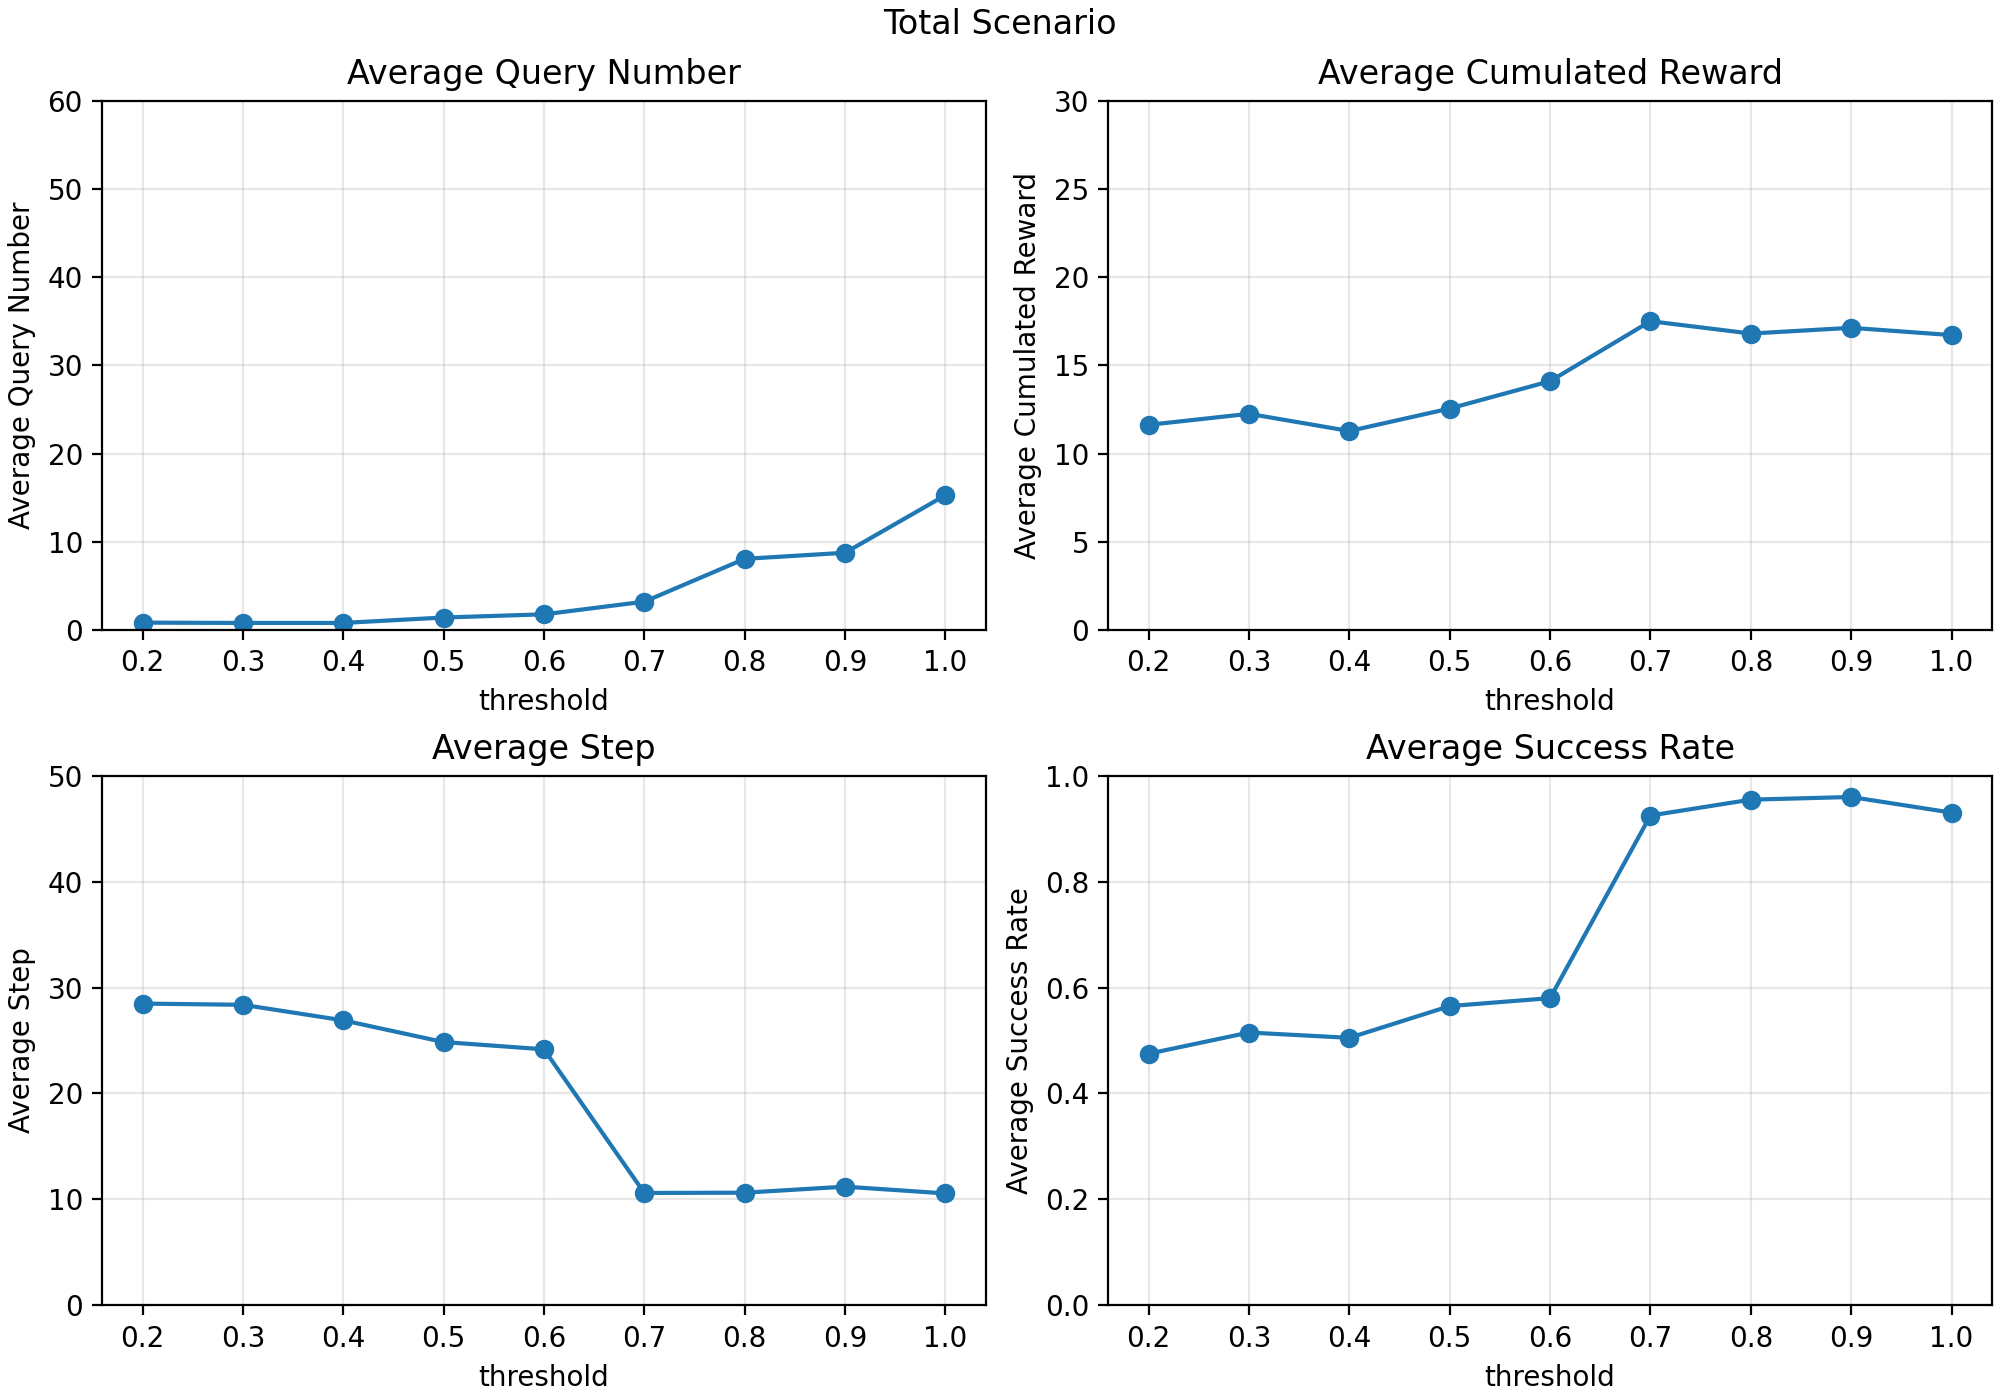
\includegraphics[width=\linewidth]{figures/tau_plots/wastesorting_total_scenario.png}
  \caption{Waste sorting}
  \label{fig:tau_total_wastesorting}
\end{subfigure}
\hfill
\begin{subfigure}[t]{0.48\linewidth}
  \centering
  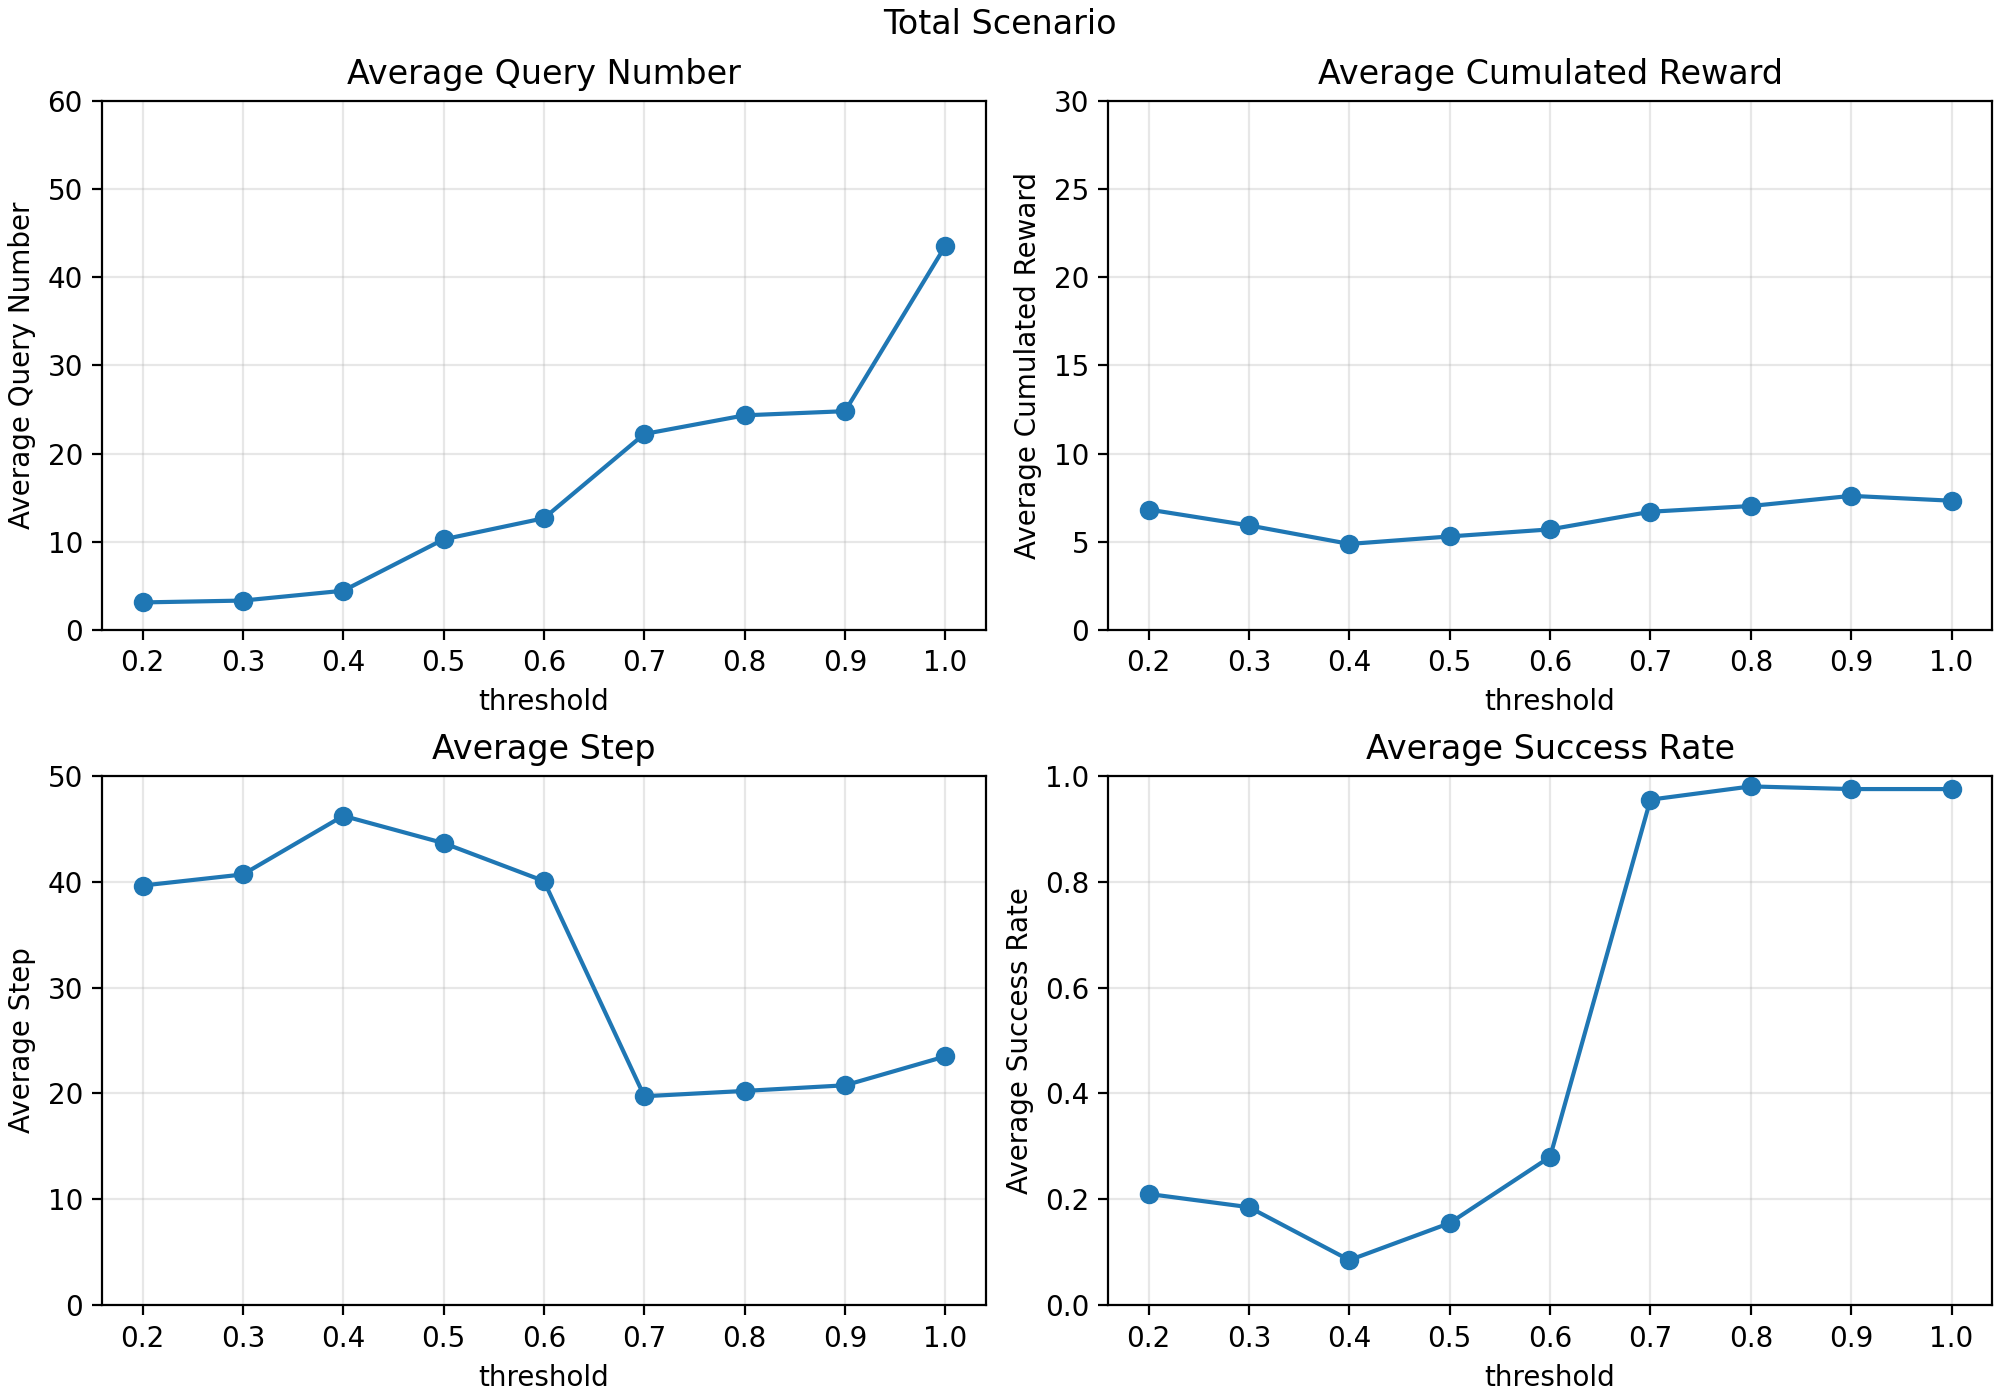
\includegraphics[width=\linewidth]{figures/tau_plots/tomato_total_scenario.png}
  \caption{Tomato harvesting}
  \label{fig:tau_total_tomato}
\end{subfigure}
\caption{Aggregate threshold analysis over all five scenarios.}
\label{fig:tau_total}
\end{figure}

\begin{figure}[H]
\centering
\begin{subfigure}[t]{0.48\linewidth}
  \centering
  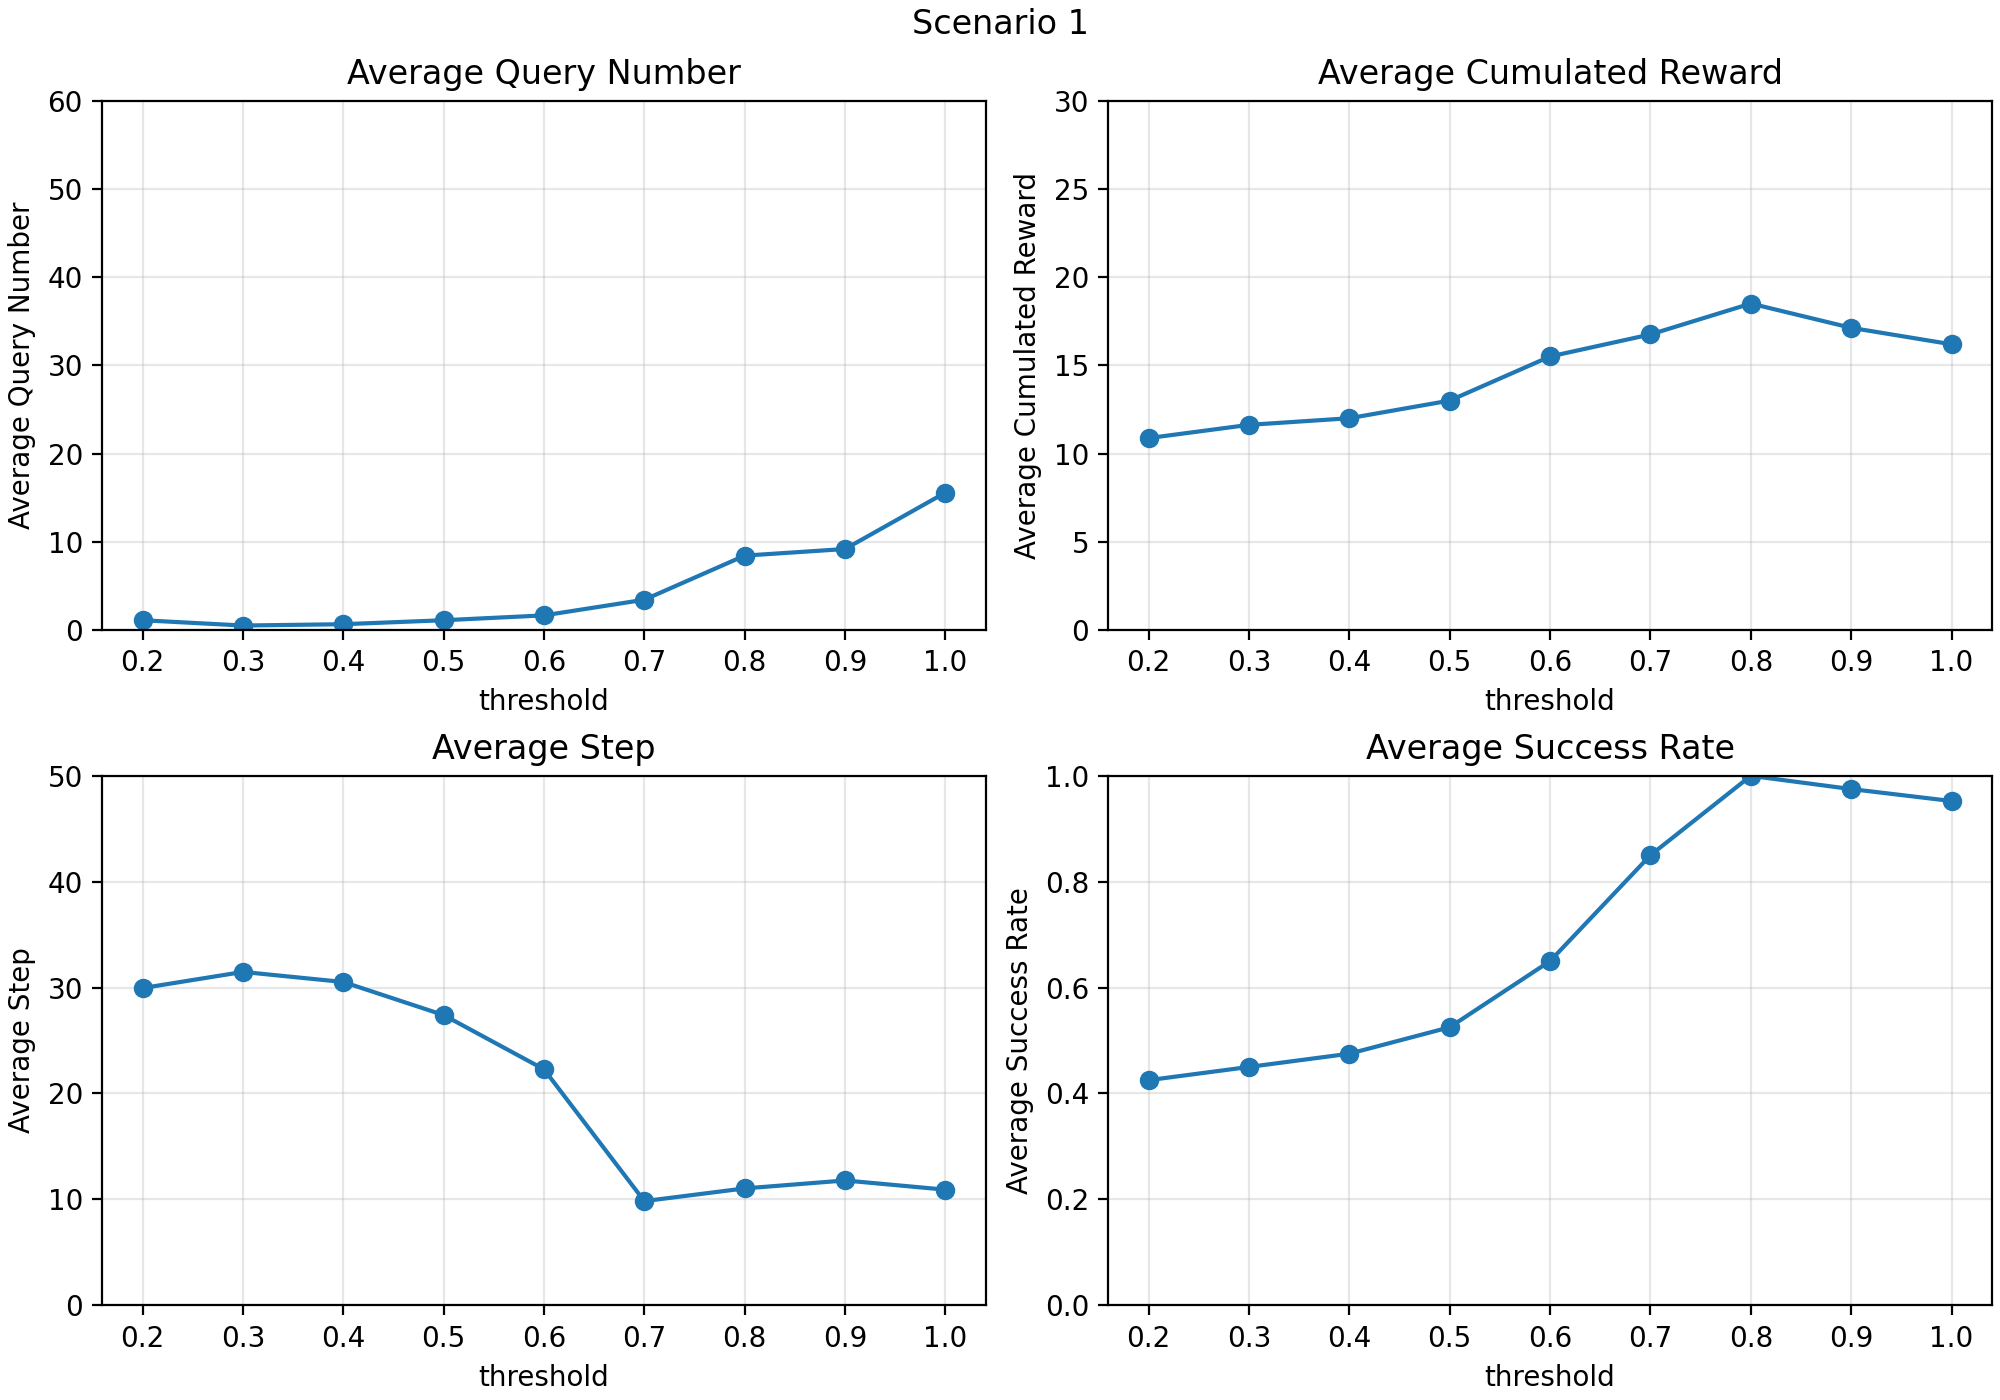
\includegraphics[width=\linewidth]{figures/tau_plots/wastesorting_scenario_1.png}
  \caption{Scenario 1}
\end{subfigure}
\hfill
\begin{subfigure}[t]{0.48\linewidth}
  \centering
  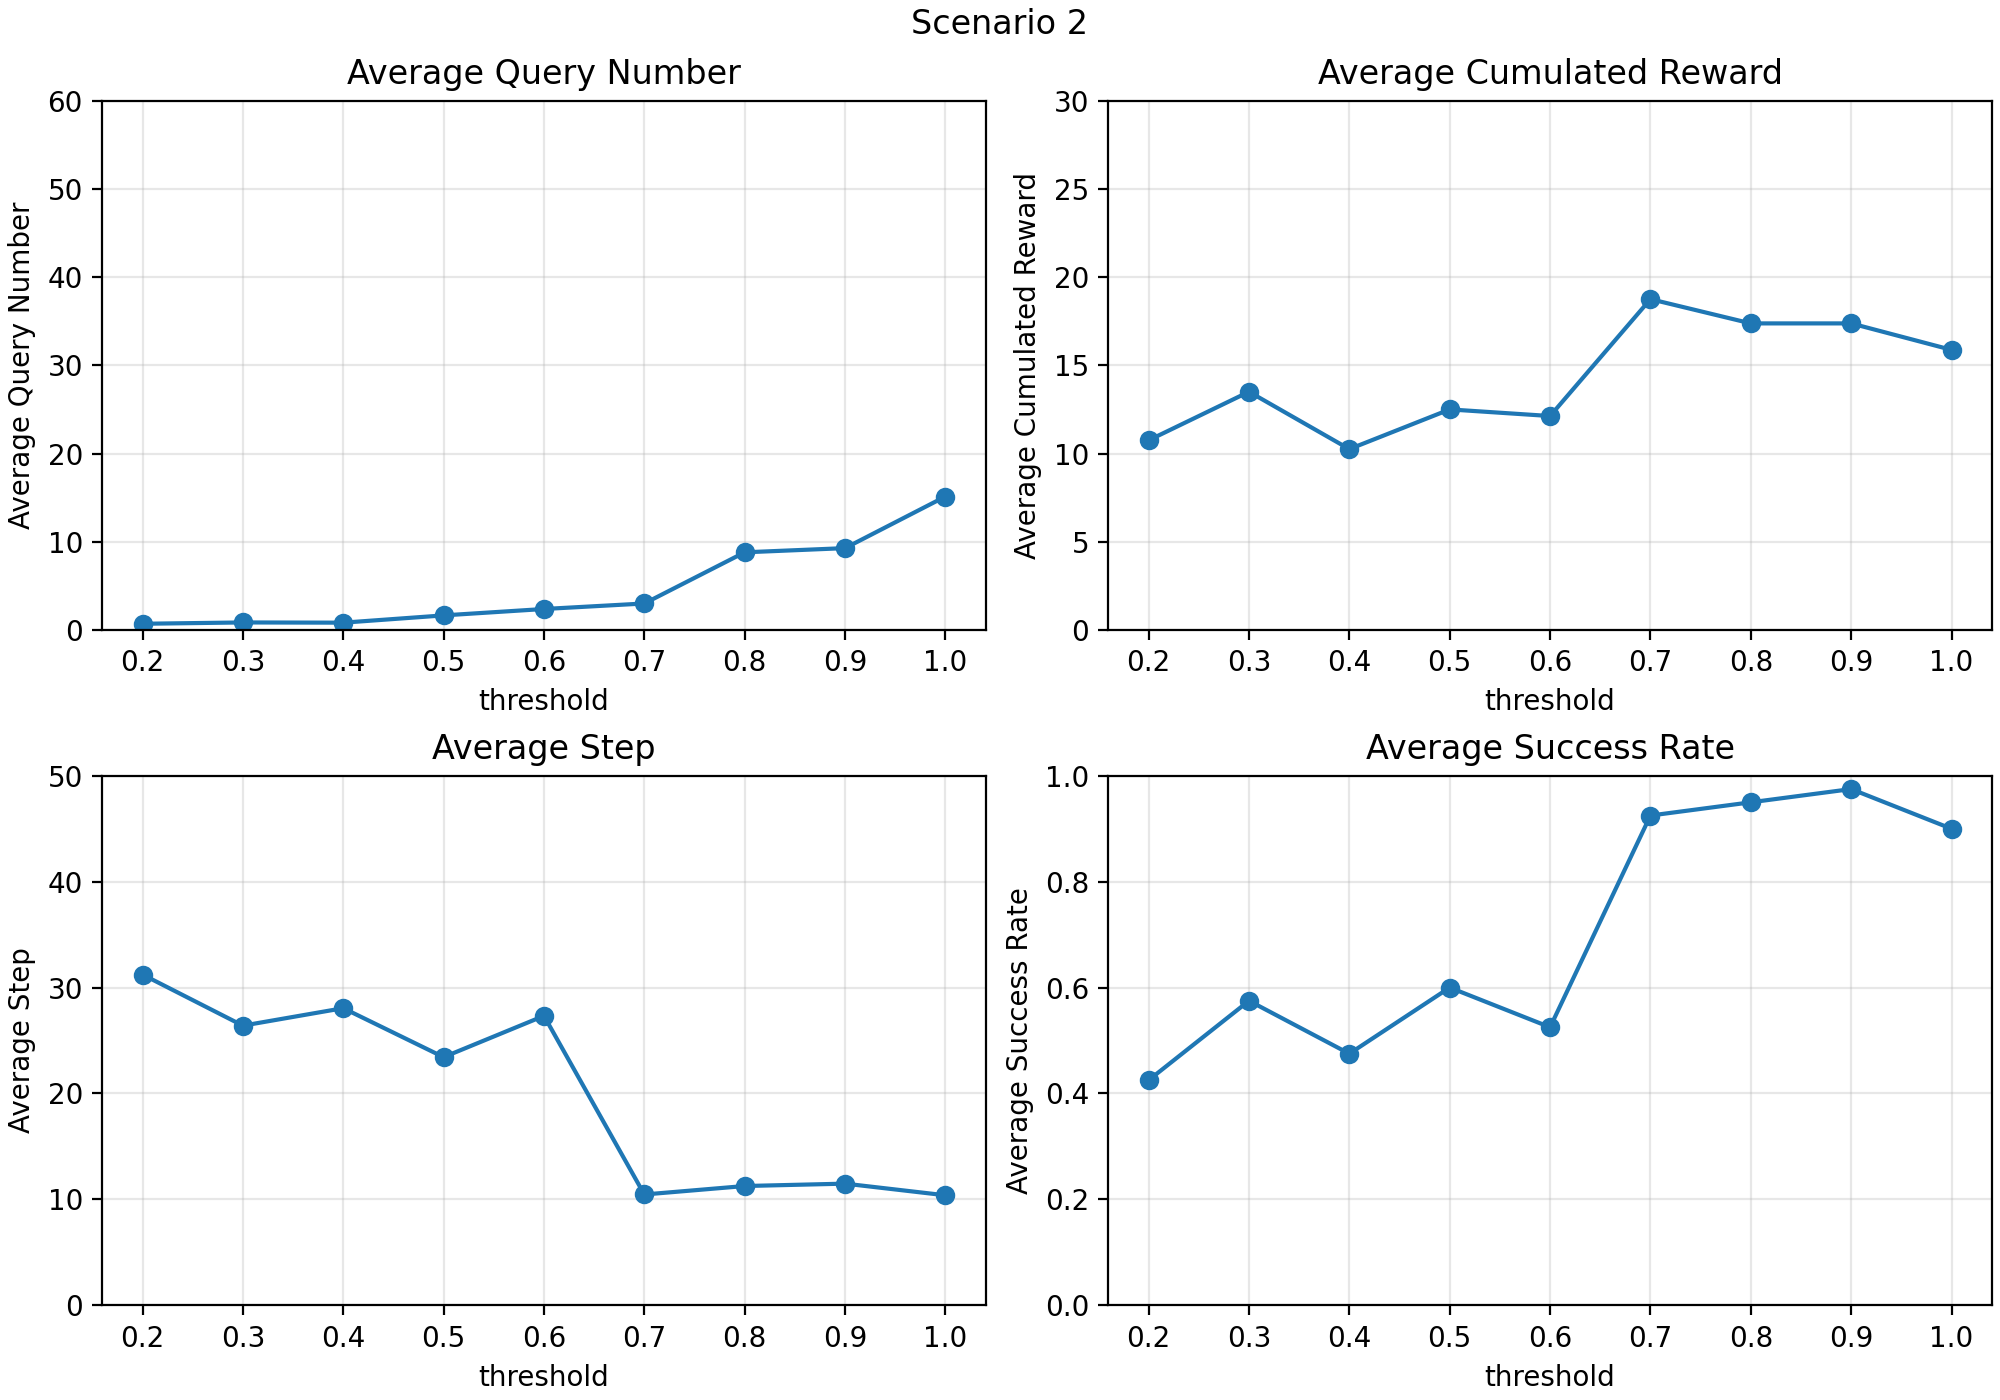
\includegraphics[width=\linewidth]{figures/tau_plots/wastesorting_scenario_2.png}
  \caption{Scenario 2}
\end{subfigure}

\begin{subfigure}[t]{0.48\linewidth}
  \centering
  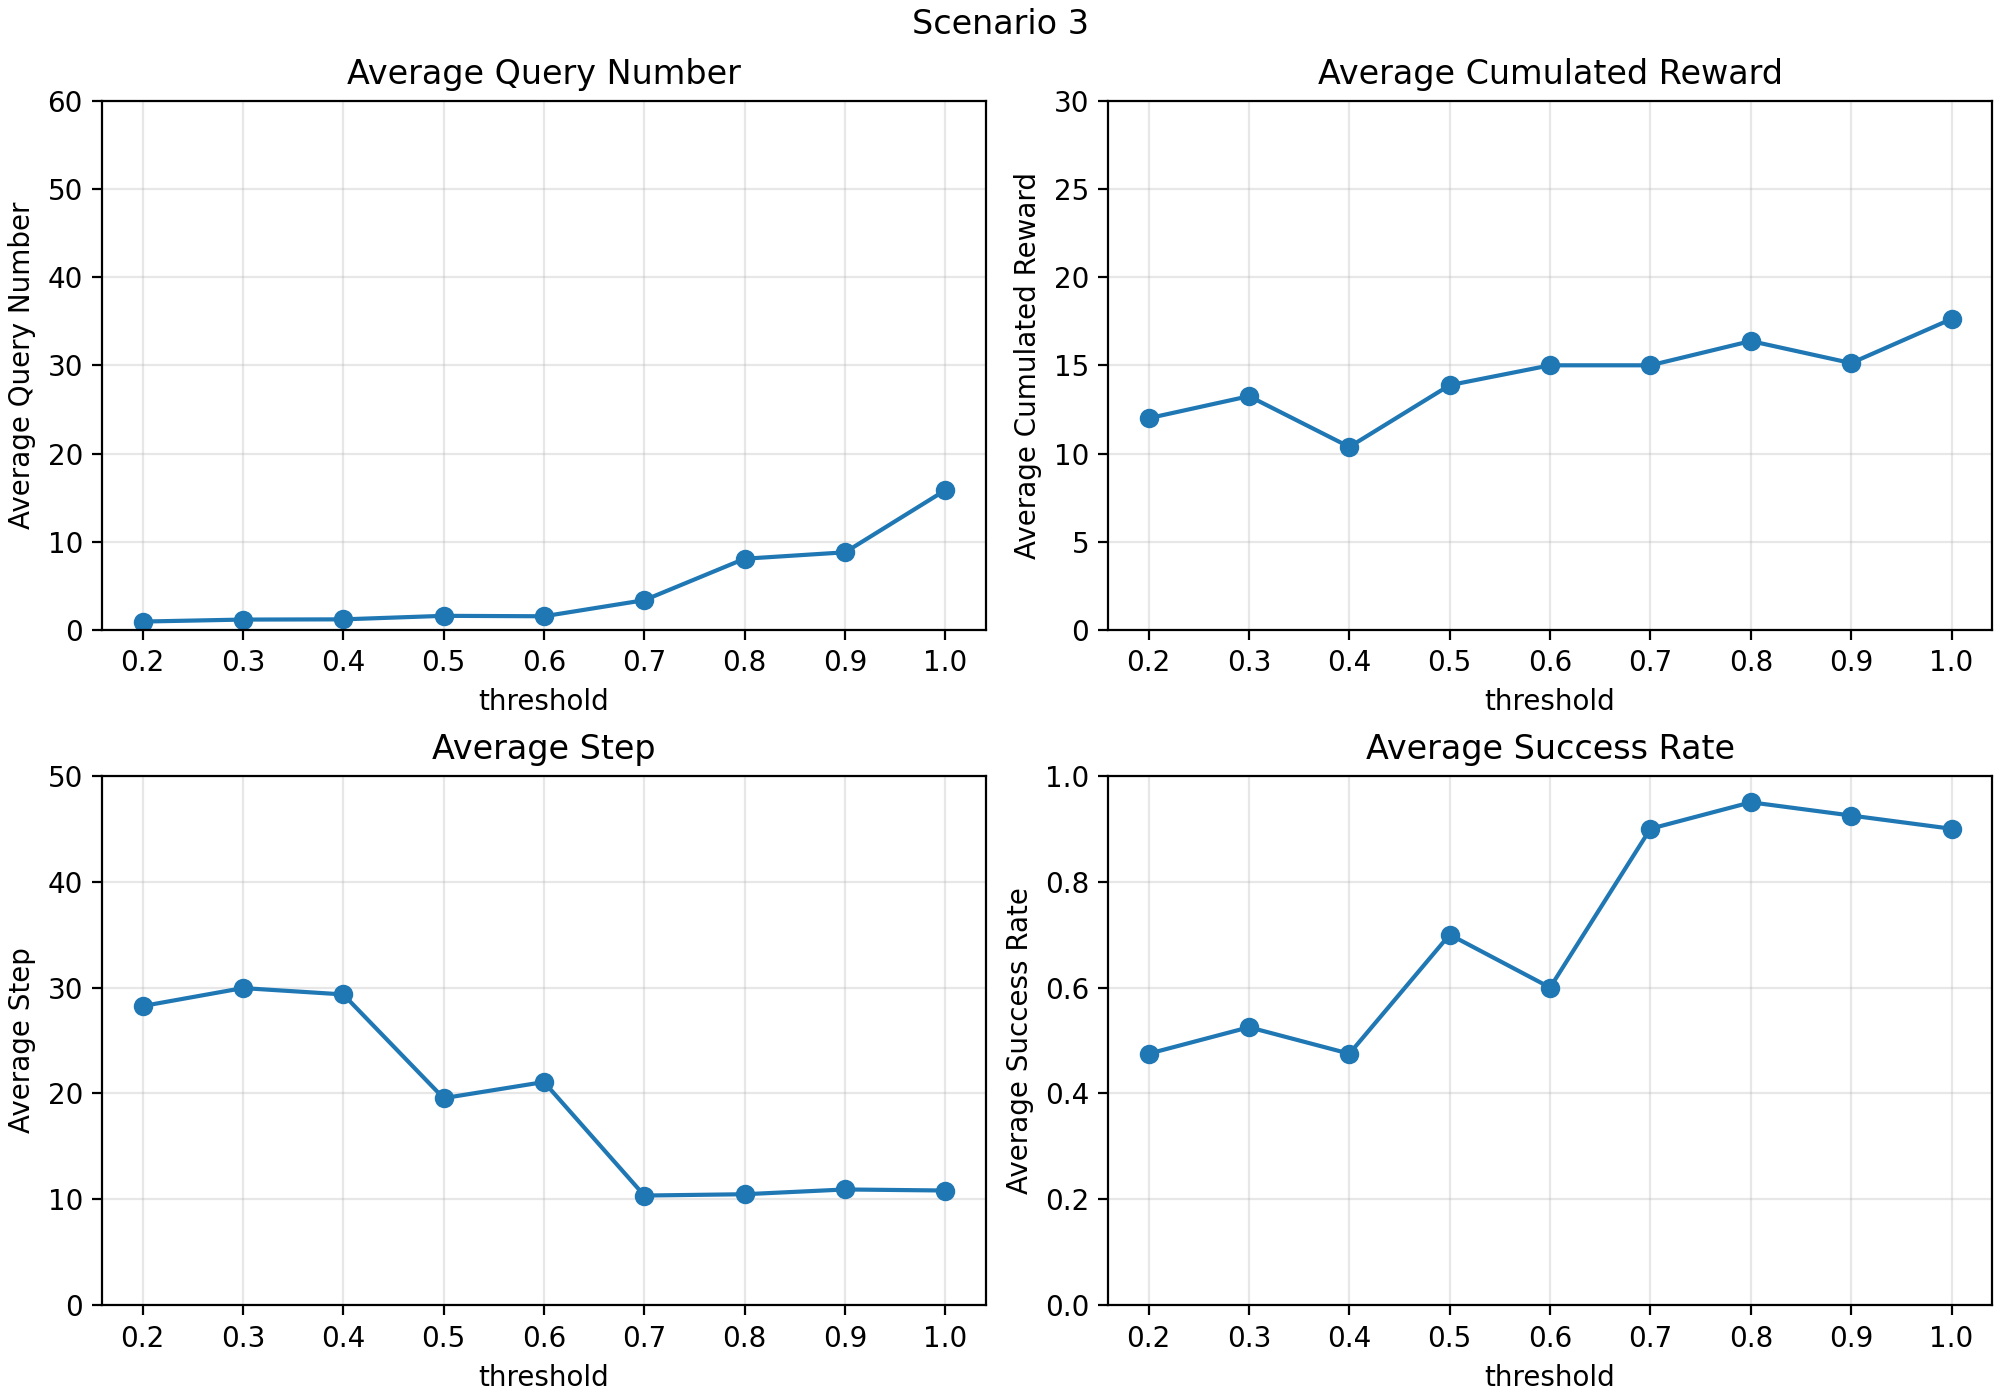
\includegraphics[width=\linewidth]{figures/tau_plots/wastesorting_scenario_3.png}
  \caption{Scenario 3}
\end{subfigure}
\hfill
\begin{subfigure}[t]{0.48\linewidth}
  \centering
  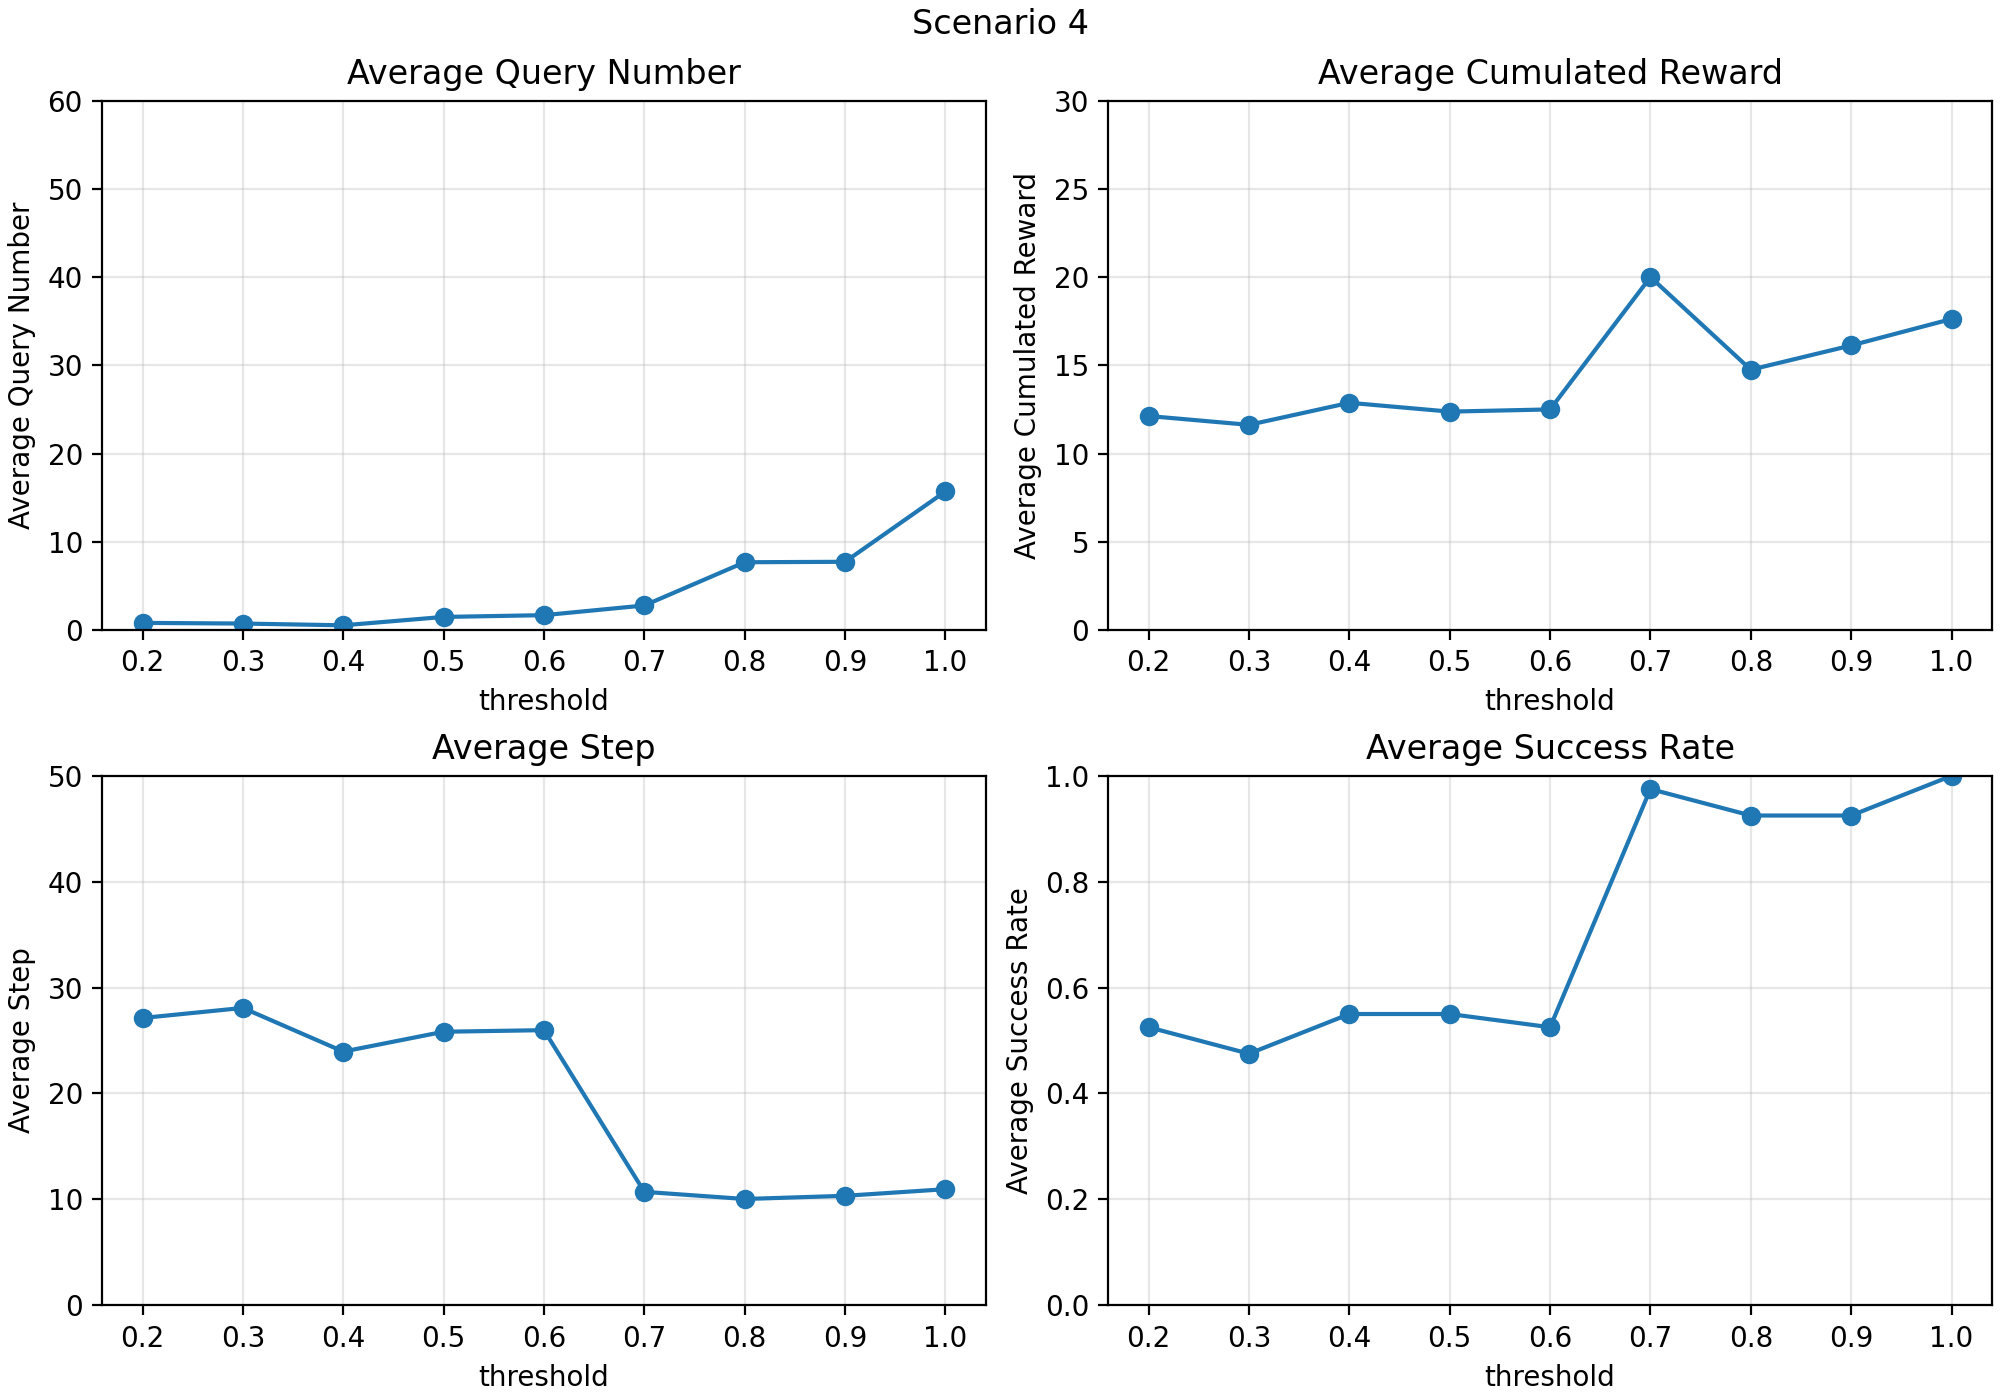
\includegraphics[width=\linewidth]{figures/tau_plots/wastesorting_scenario_4.png}
  \caption{Scenario 4}
\end{subfigure}

\begin{subfigure}[t]{0.48\linewidth}
  \centering
  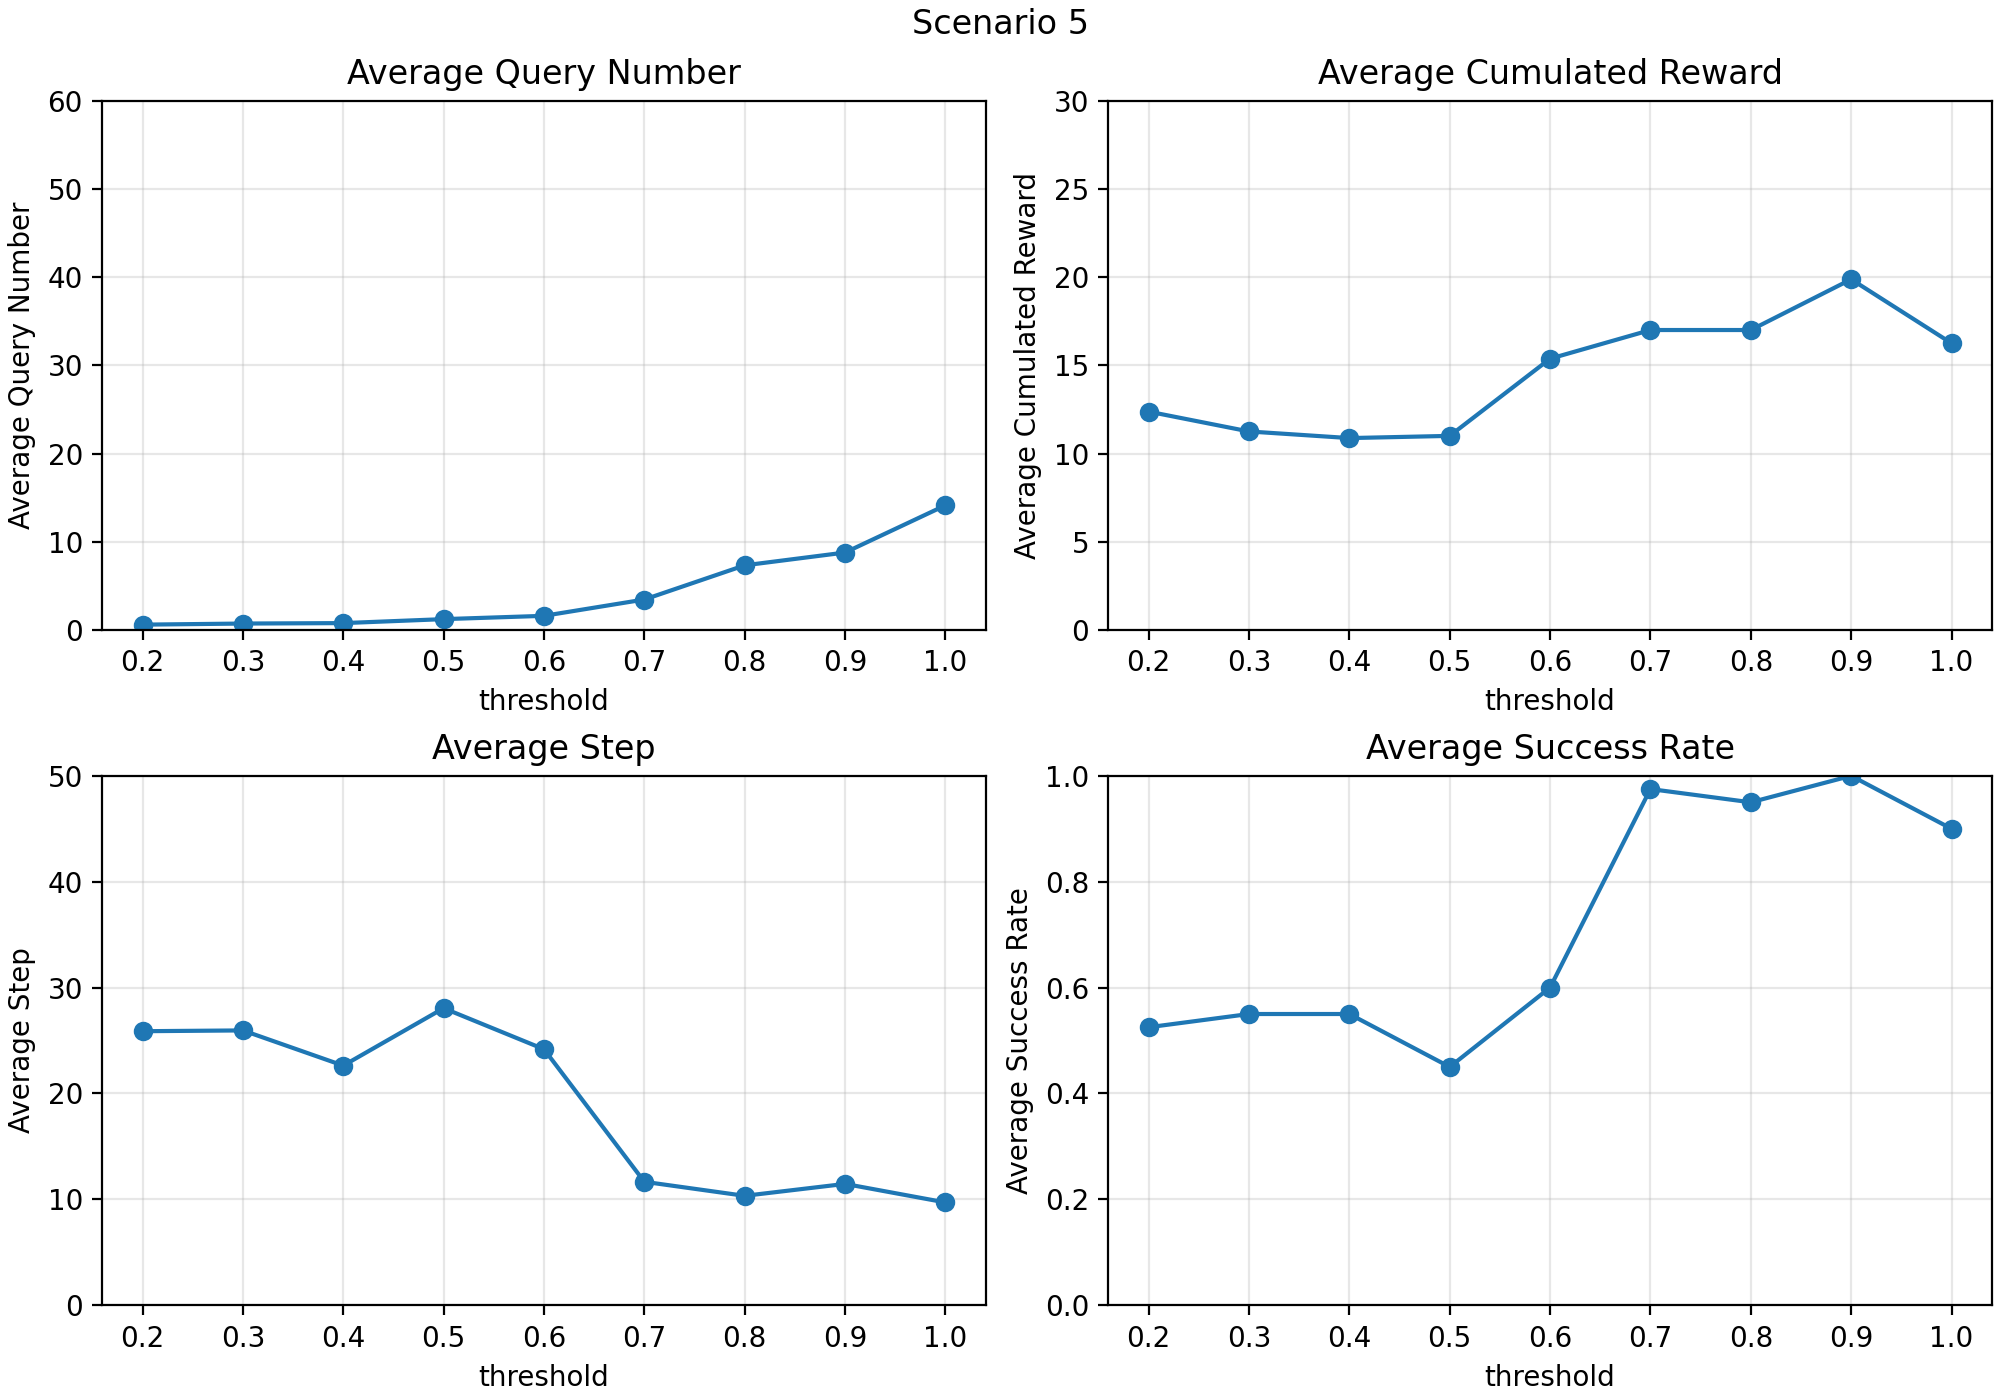
\includegraphics[width=\linewidth]{figures/tau_plots/wastesorting_scenario_5.png}
  \caption{Scenario 5}
\end{subfigure}
\caption{Threshold analysis for individual waste sorting scenarios.}
\label{fig:tau_wastesorting_scenarios}
\end{figure}

\begin{figure}[H]
\centering
\begin{subfigure}[t]{0.48\linewidth}
  \centering
  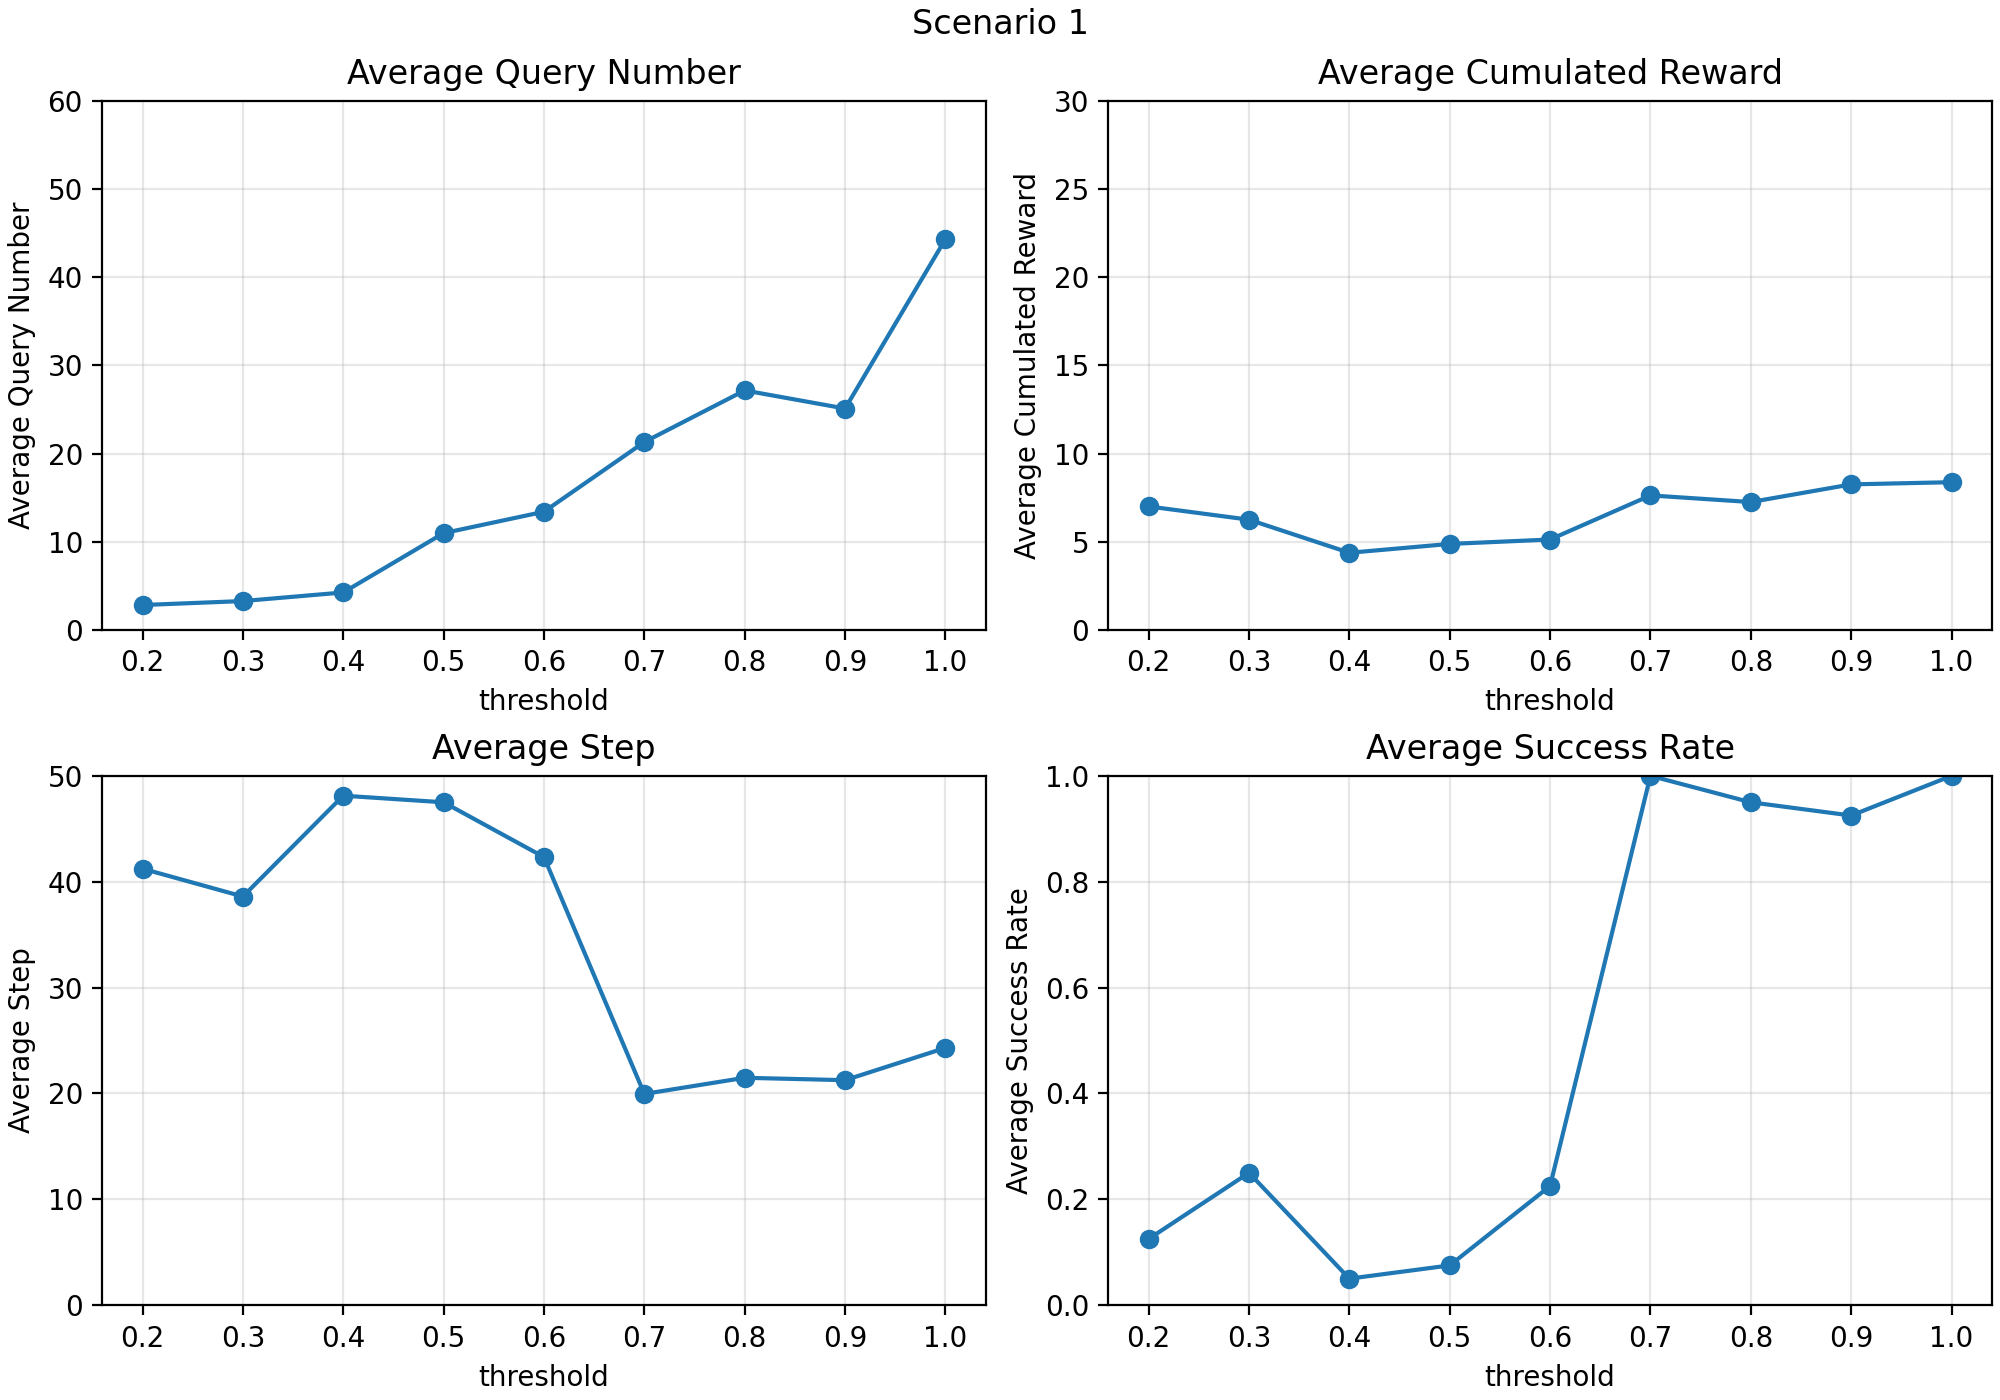
\includegraphics[width=\linewidth]{figures/tau_plots/tomato_scenario_1.png}
  \caption{Scenario 1}
\end{subfigure}
\hfill
\begin{subfigure}[t]{0.48\linewidth}
  \centering
  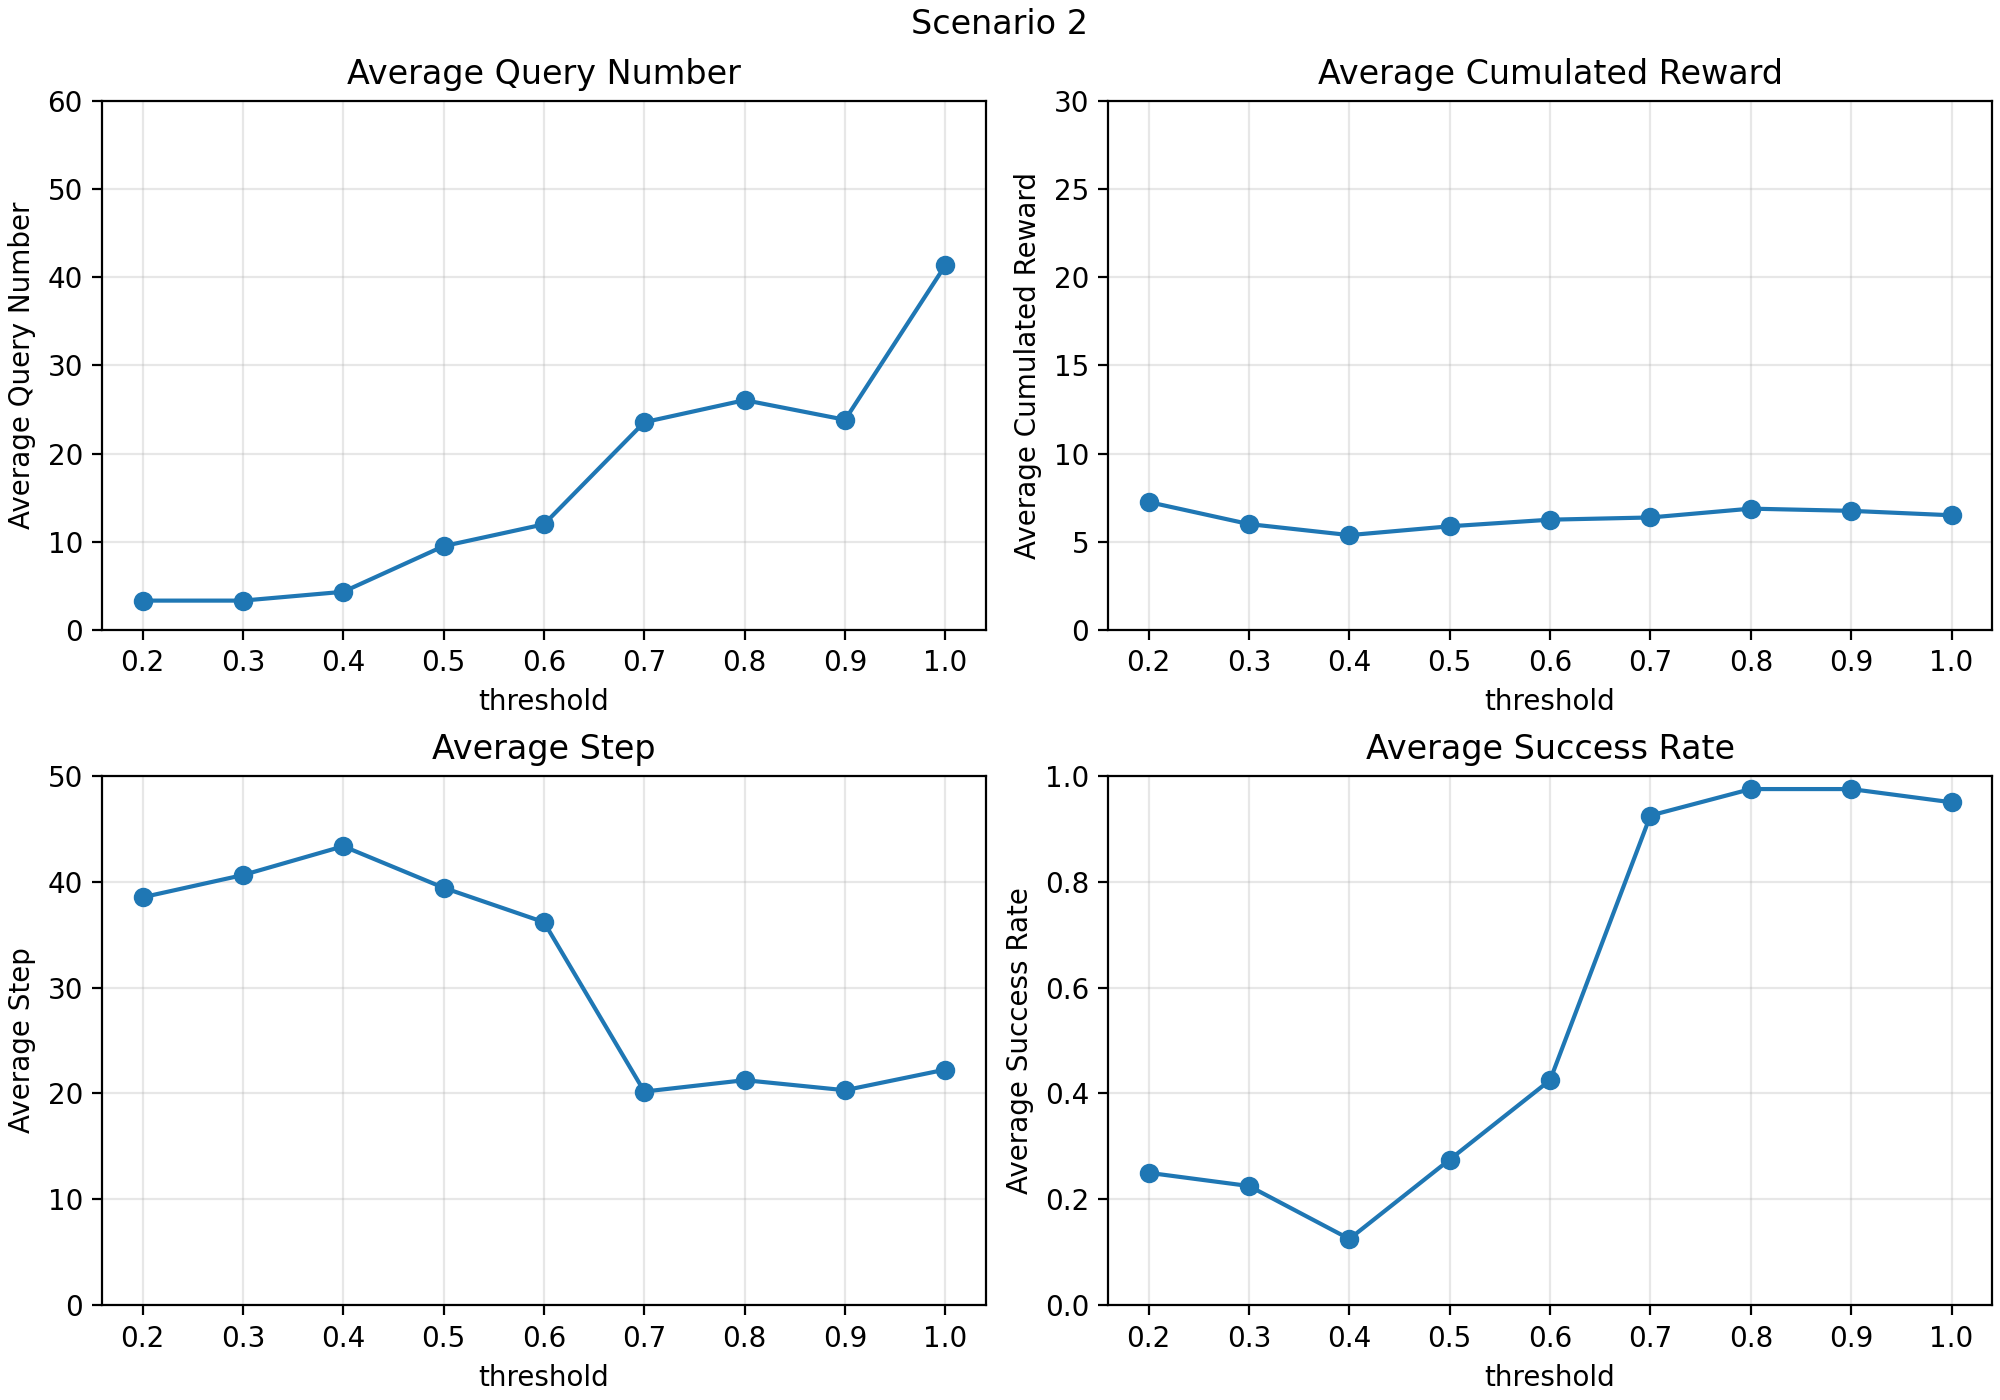
\includegraphics[width=\linewidth]{figures/tau_plots/tomato_scenario_2.png}
  \caption{Scenario 2}
\end{subfigure}

\begin{subfigure}[t]{0.48\linewidth}
  \centering
  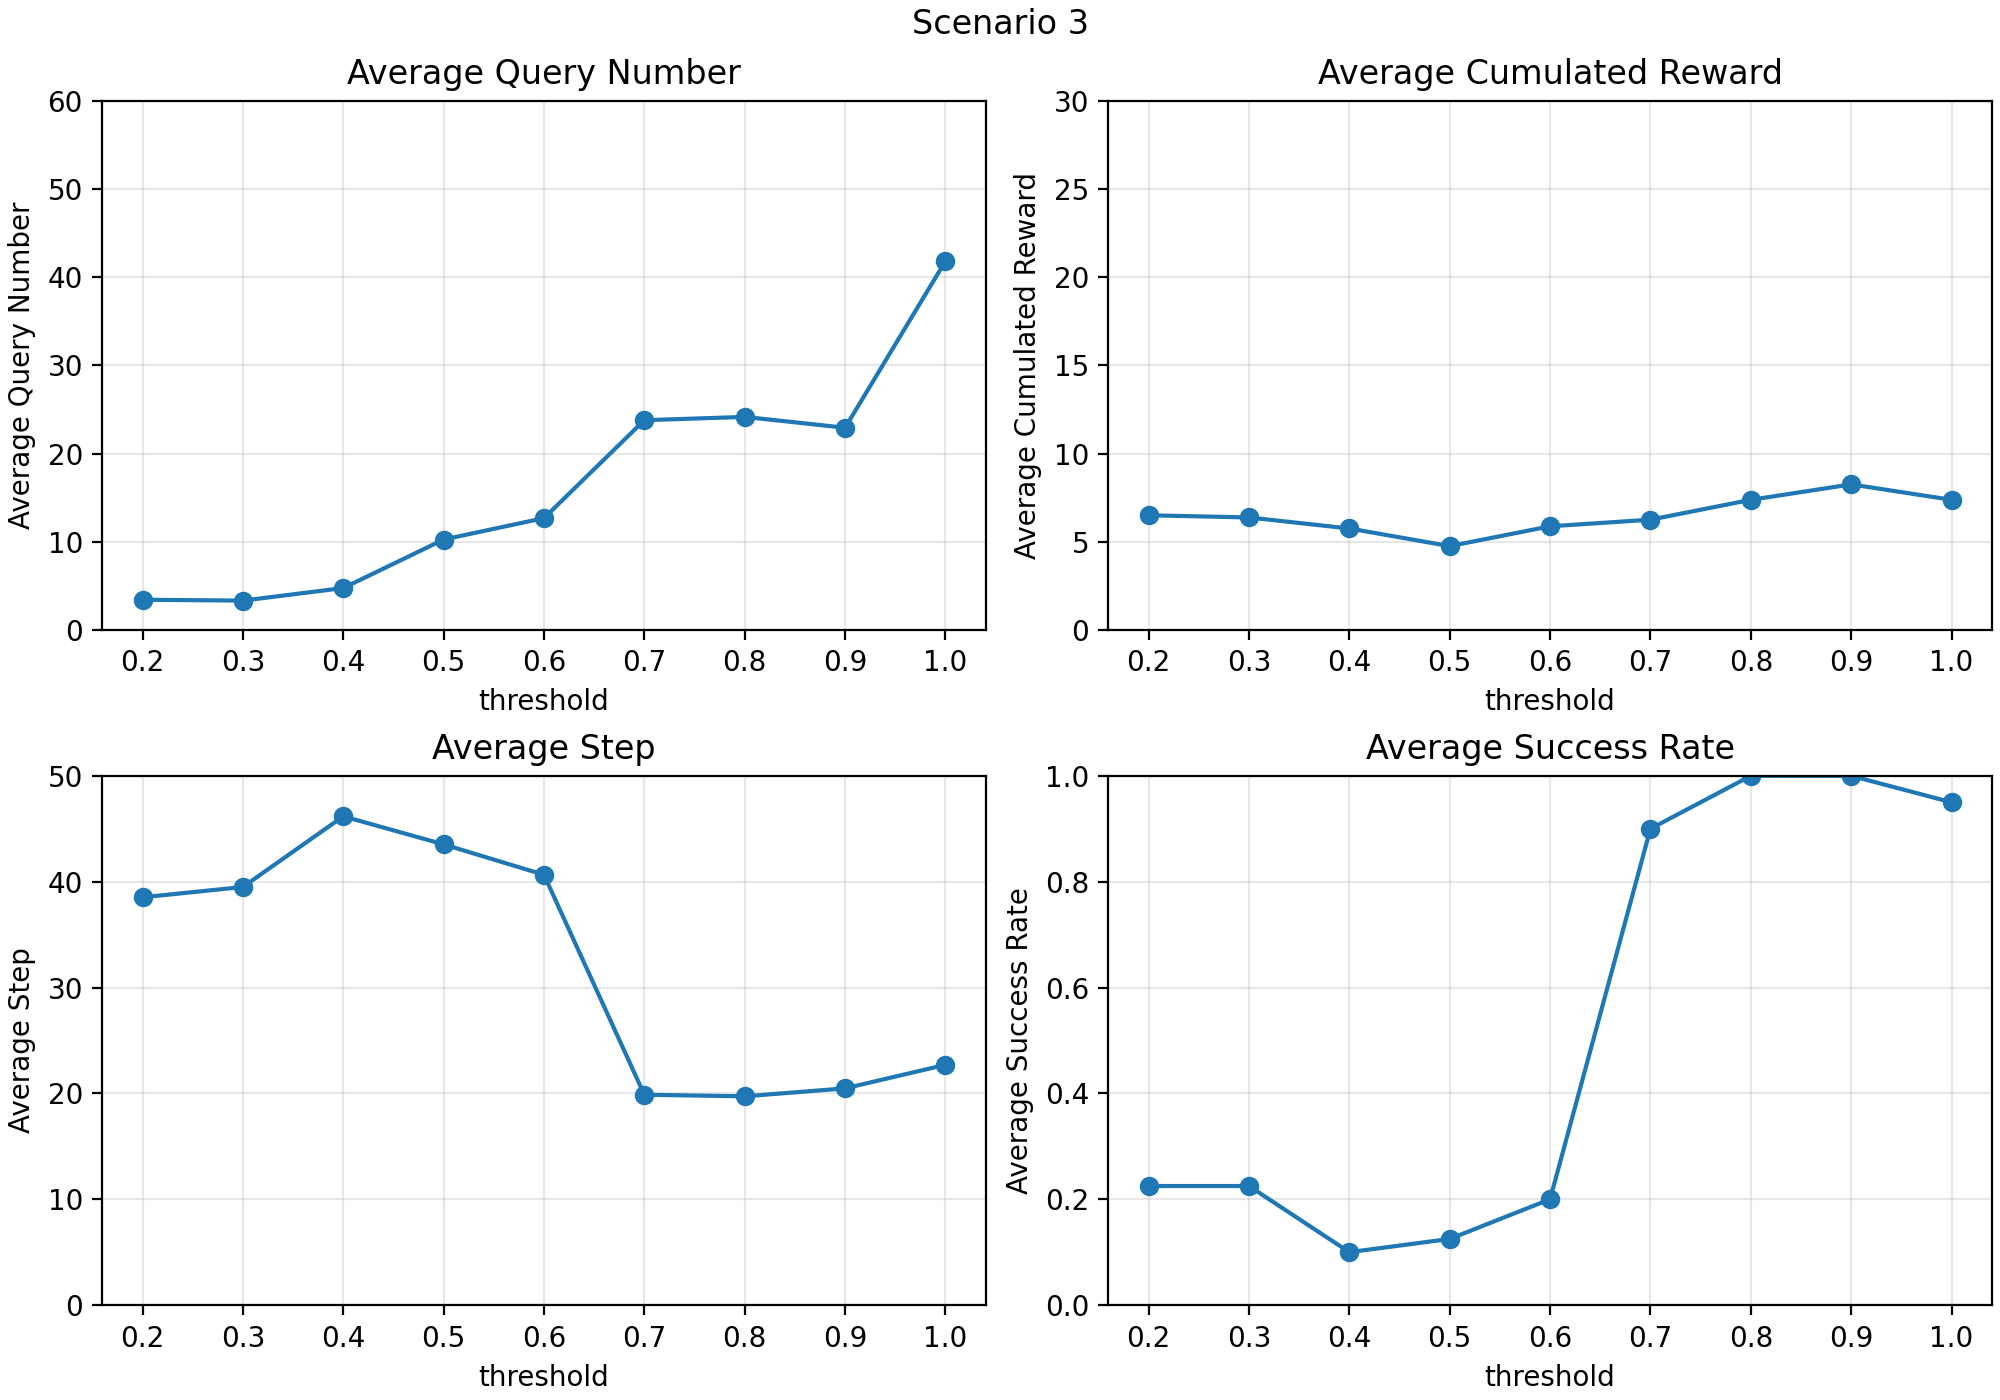
\includegraphics[width=\linewidth]{figures/tau_plots/tomato_scenario_3.png}
  \caption{Scenario 3}
\end{subfigure}
\hfill
\begin{subfigure}[t]{0.48\linewidth}
  \centering
  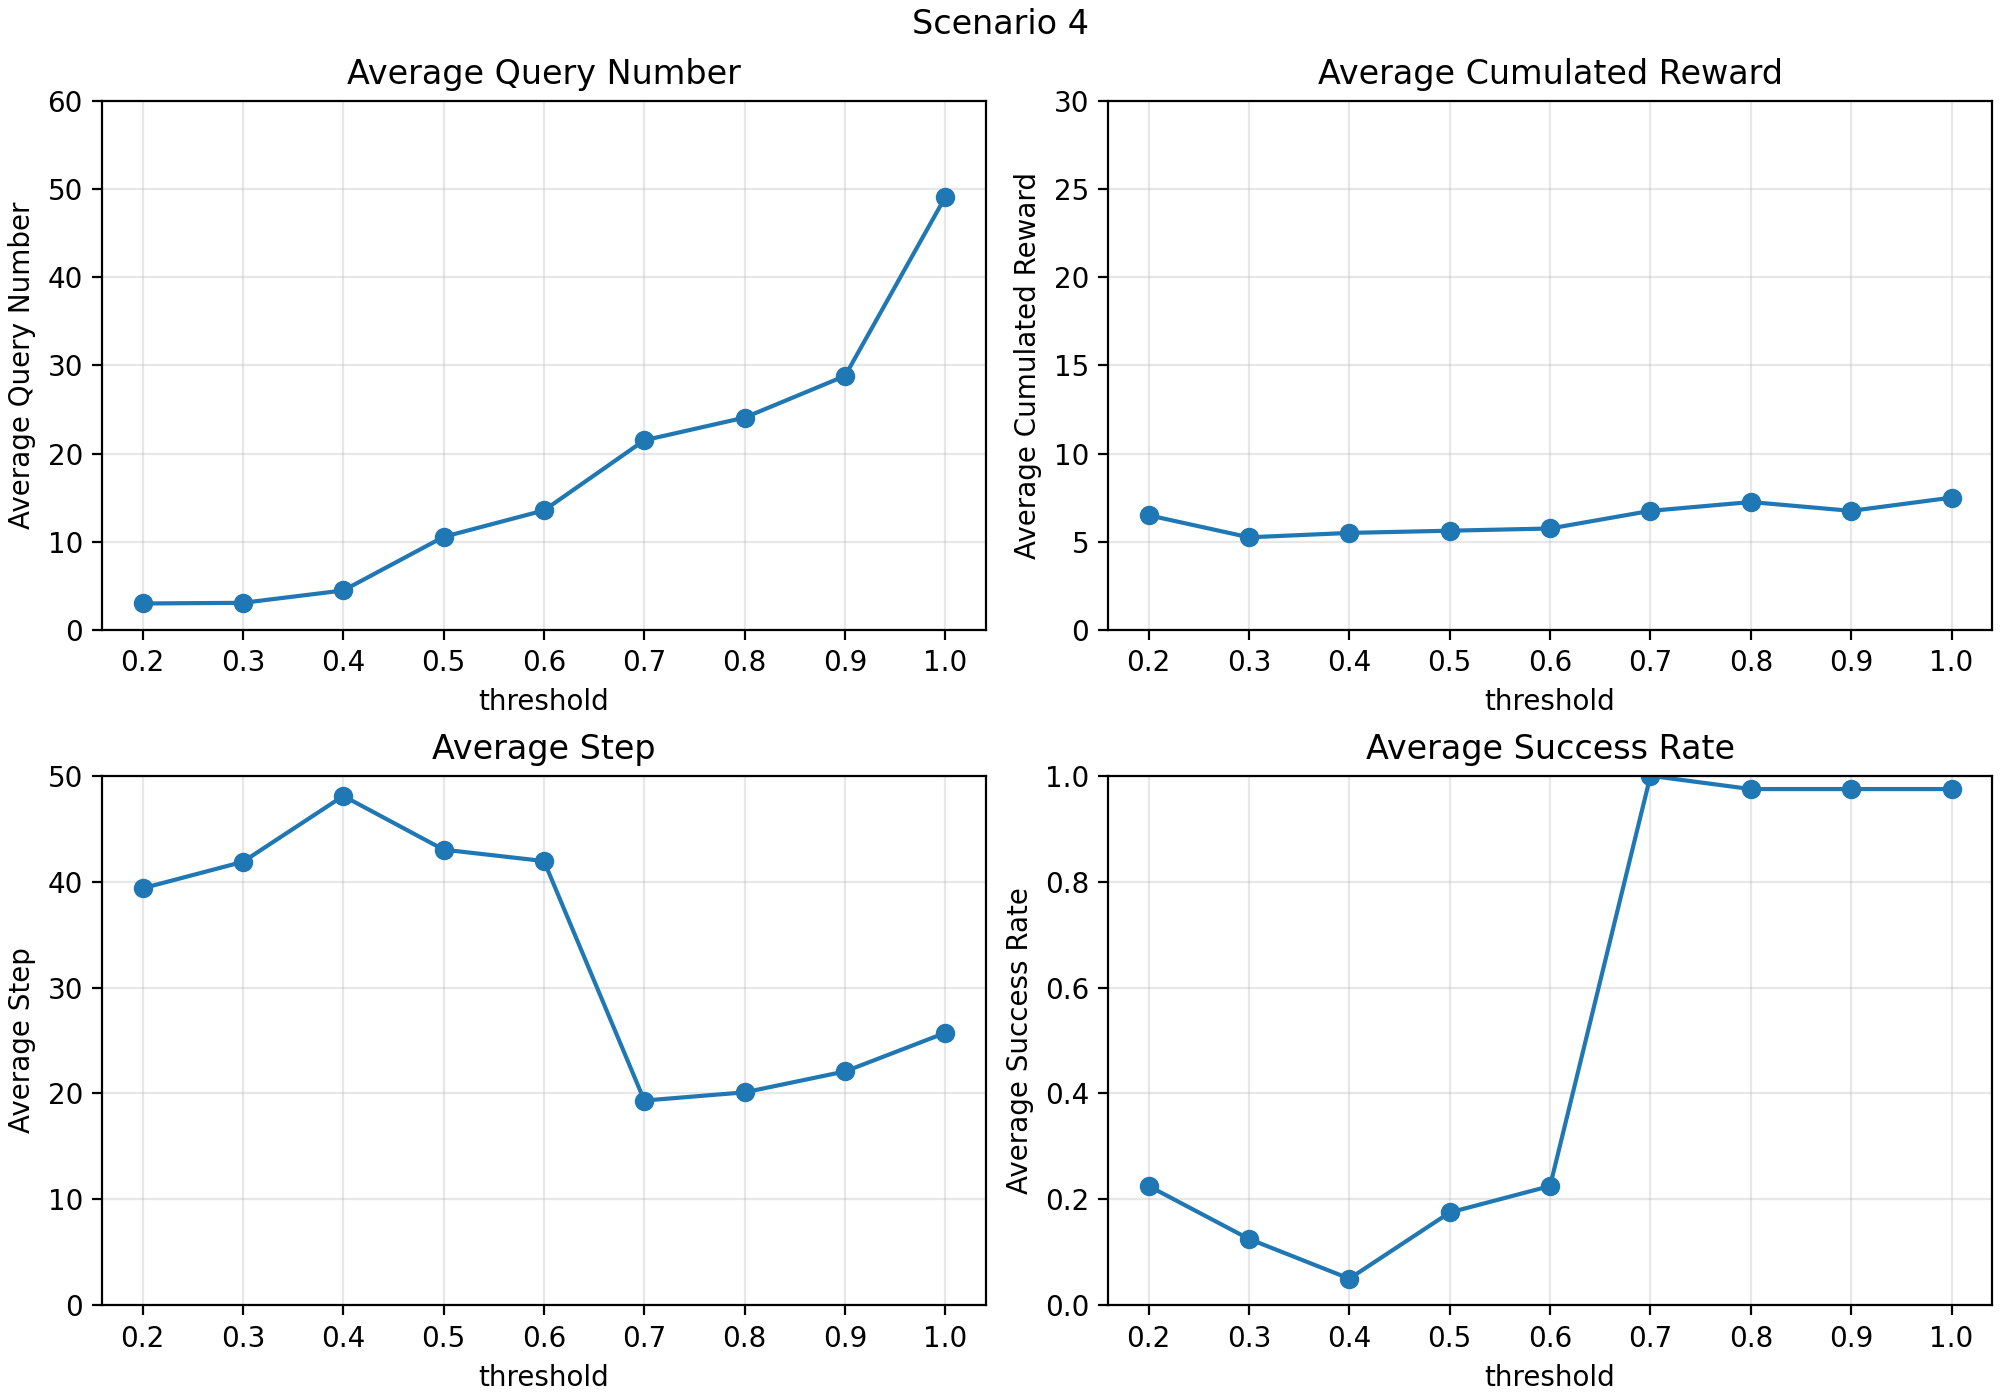
\includegraphics[width=\linewidth]{figures/tau_plots/tomato_scenario_4.png}
  \caption{Scenario 4}
\end{subfigure}

\begin{subfigure}[t]{0.48\linewidth}
  \centering
  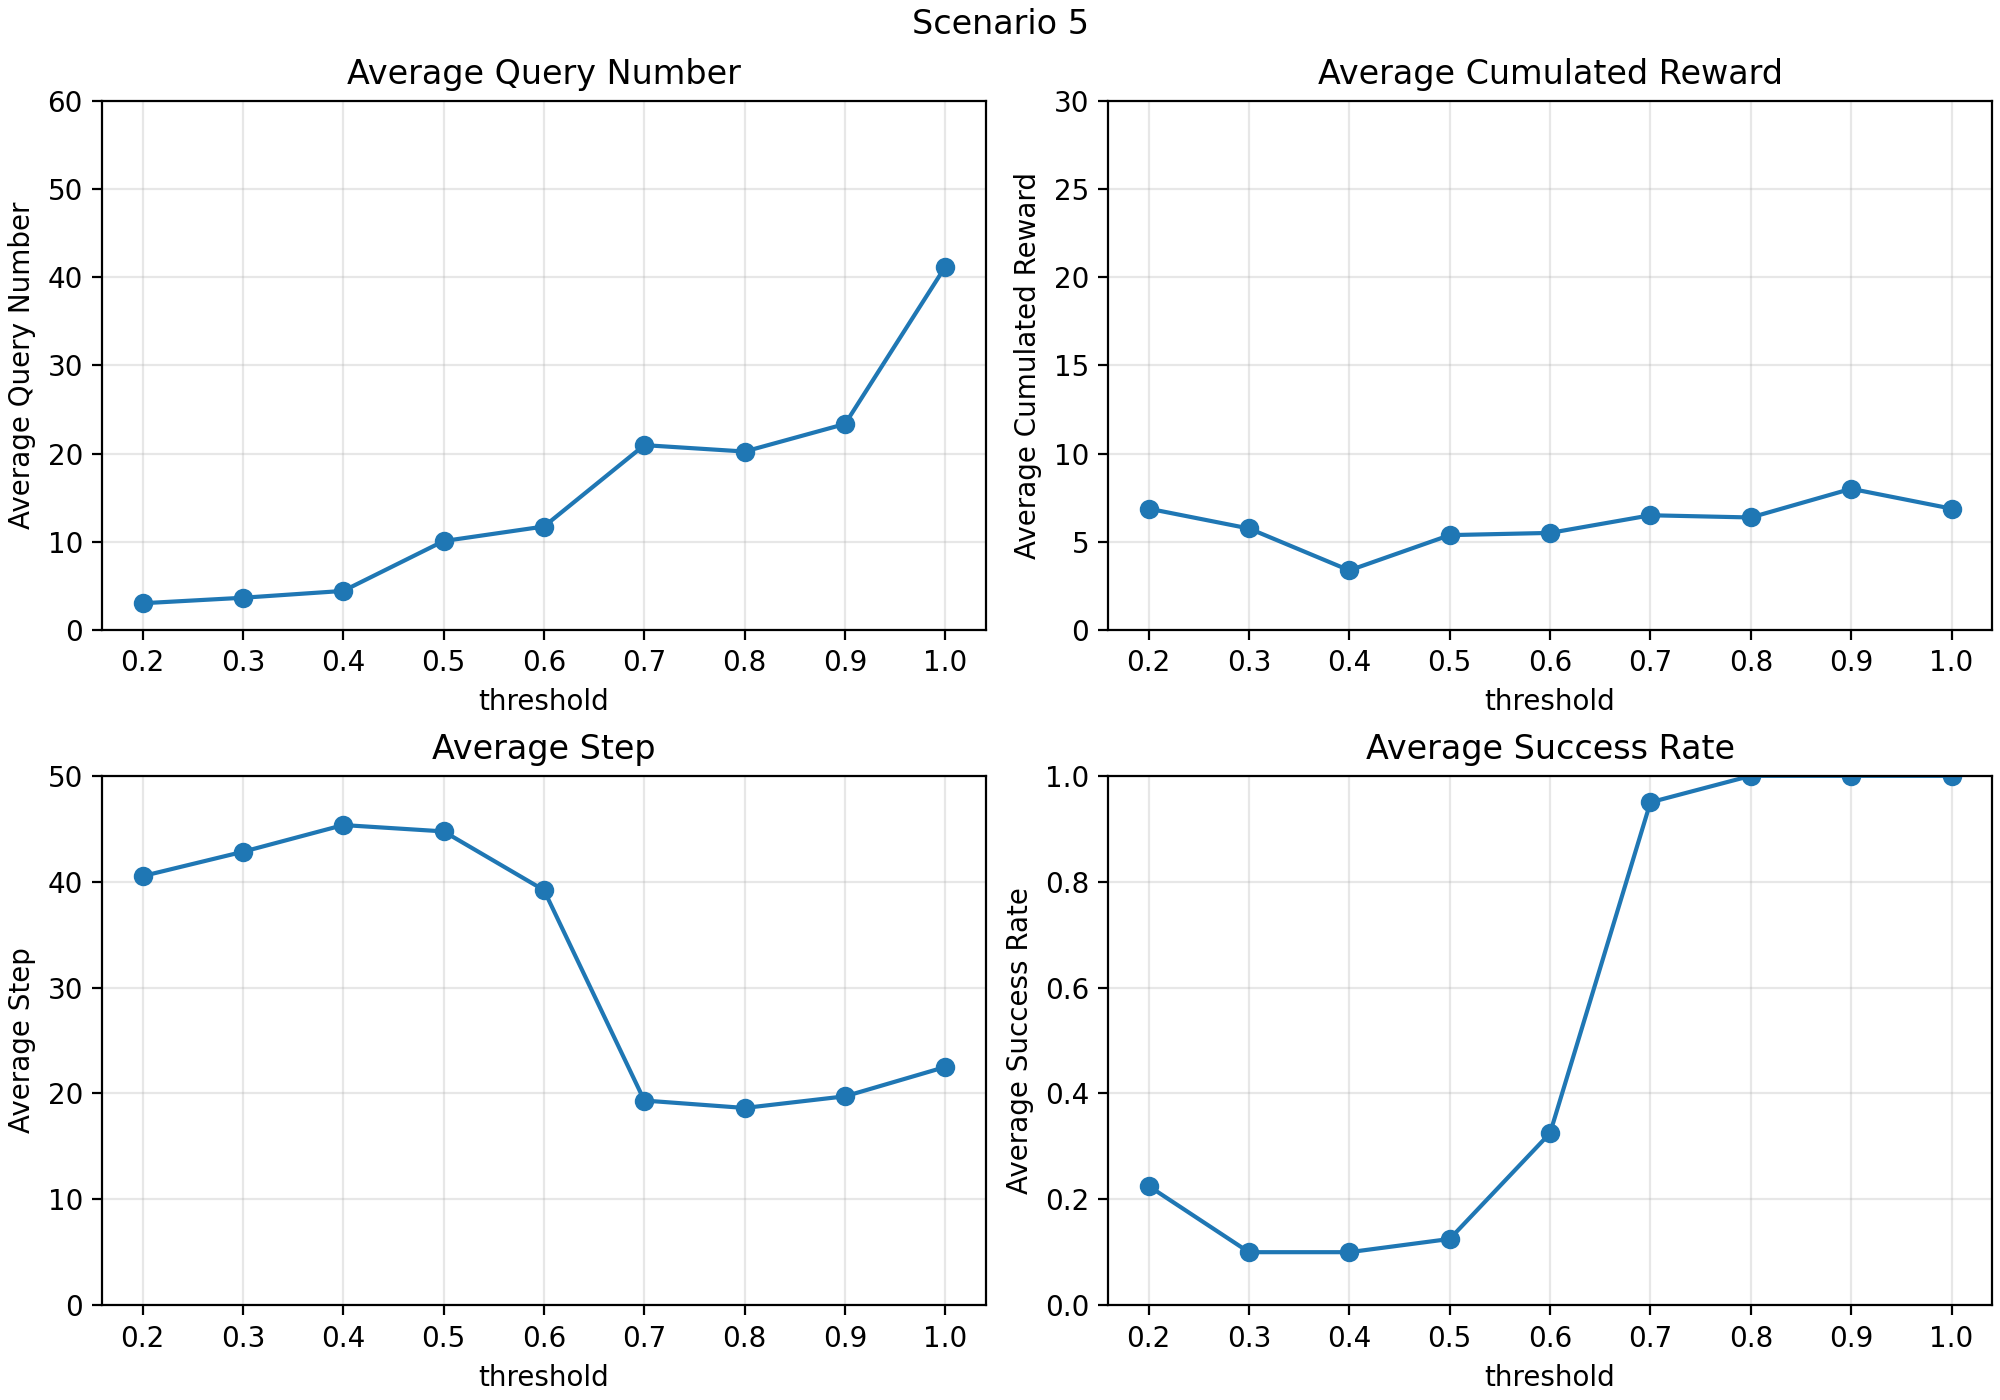
\includegraphics[width=\linewidth]{figures/tau_plots/tomato_scenario_5.png}
  \caption{Scenario 5}
\end{subfigure}
\caption{Threshold analysis for individual tomato harvesting scenarios.}
\label{fig:tau_tomato_scenarios}
\end{figure}
